\documentclass[border=3pt,tikz]{standalone}
% Shared look for every TikZ figure in these notes.
% Included by each standalone figure file; also keeps the figures consistent
% with the colours used in the PDF and on the website.

\usepackage{tikz}
\usepackage{pgfplots}
\pgfplotsset{compat=1.18}
\usetikzlibrary{arrows.meta, decorations.markings, decorations.pathmorphing,
                patterns, calc, positioning}
\usepackage{amsmath}

% Series colours are the three validated categorical slots also used by the
% interactive widgets, so a path drawn in the printed notes and the same path on
% the website are the same colour. They clear the colour-vision-deficiency and
% contrast checks as a set; every path is direct-labelled as well, so colour is
% never the only thing carrying identity.
\definecolor{duPurple}{HTML}{68246D}
\definecolor{duBlue}{HTML}{2A78D6}
\definecolor{duRed}{HTML}{EB6834}
\definecolor{duGreen}{HTML}{1BAF7A}
\definecolor{duGrey}{HTML}{6B6B6B}

\tikzset{
  axisline/.style   = {-{Stealth[length=3mm]}, line width=0.7pt, black},
  path1/.style      = {duBlue,   line width=1.1pt},
  path2/.style      = {duRed,    line width=1.1pt},
  path3/.style      = {duGreen,  line width=1.1pt},
  statedot/.style   = {circle, fill=black, inner sep=1.4pt},
  arrowhead/.style  = {decoration={markings,
                        mark=at position #1 with {\arrow{Stealth[length=2.6mm]}}},
                       postaction={decorate}},
  lbl/.style        = {font=\small},
  slbl/.style       = {font=\footnotesize, duGrey},
  workfill/.style   = {duPurple, opacity=0.16},
}

\usetikzlibrary{shapes.geometric}
% Clausius inequality: reversible and irreversible engines with the same Q_H
\begin{document}
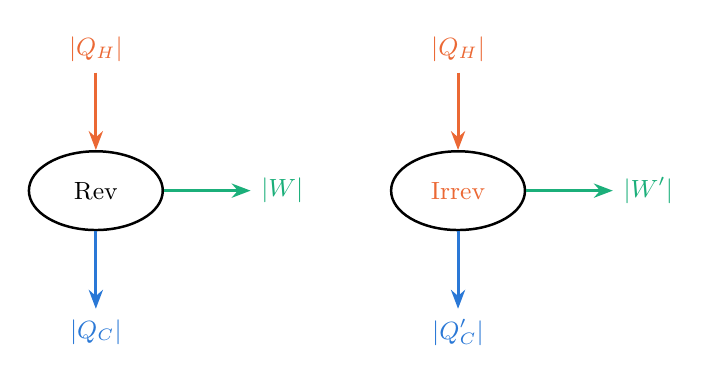
\begin{tikzpicture}[x=1cm,y=1cm,
    eng/.style={ellipse, draw=black, line width=0.9pt, minimum width=1.7cm, minimum height=1.0cm, font=\small},
    flow/.style={-{Stealth[length=2.4mm]}, line width=1.1pt}]
  \foreach \x/\name/\w/\qc in {0/Rev/{W}/{Q_C}, 4.6/{\textcolor{duRed}{Irrev}}/{W'}/{Q_C'}} {
    \node[eng] (E) at (\x,0) {\name};
    \draw[flow, duRed] (\x,1.5) node[above, lbl] {$|Q_H|$} -- (E.north);
    \draw[flow, duBlue] (E.south) -- (\x,-1.5) node[below, lbl] {$|\qc|$};
    \draw[flow, duGreen] (E.east) -- ++(1.1,0) node[right, lbl] {$|\w|$};
  }
\end{tikzpicture}
\end{document}
